\section{2点関数}
\subsection{シュウィンガー・ダイソン方程式}
\begin{figure}[ht]
  \centering
  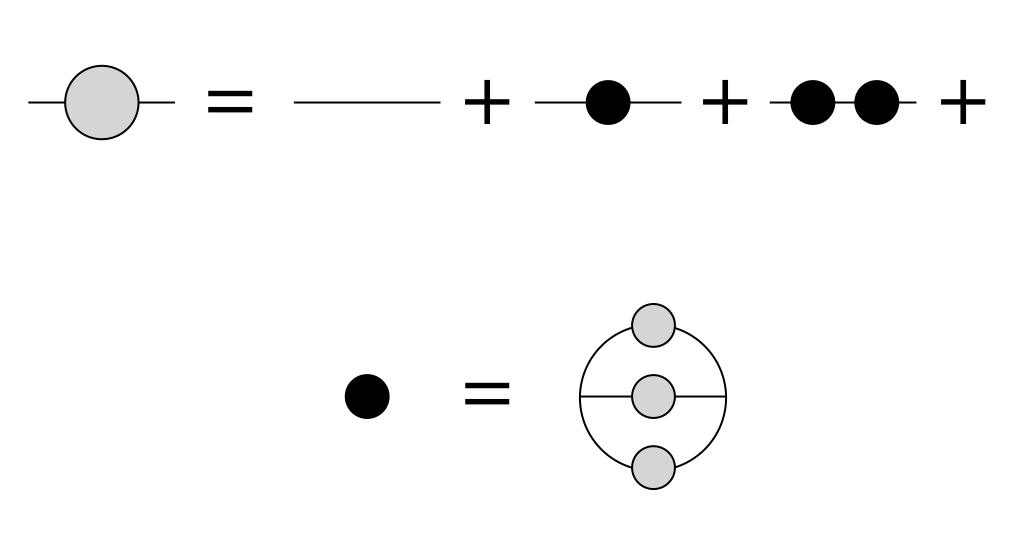
\includegraphics[width=14cm]{figures/melonDiagram}
  \caption{ラージN極限において2点関数に寄与する最初の補正ダイアグラム.
  特に$q=4$の場合について描画している. 灰色の丸と黒い丸はそれぞれ完全な2点関数および
  1粒子相互作用を表している.}
  \label{fig:melonDiagram}
\end{figure}

SYK模型の作用は
\begin{align}
  I = \int dt\ \left(\frac{1}{2}\sum_{i = 1}^{N} \psi_i \deriv \psi_i
		- \frac{1}{4!} \sum_{i,j,k,l = 1}^{N} J_{ijkl} \psi_i\psi_j\psi_k\psi_l
    \right)
\end{align}
である。
これを$J_{ijkl}$について期待値を取り、その後フェルミオンを積分するために
2つのbi-local場$G(t_1, t_2)$, $\Sigma(t_1, t_2)$を導入すると
\begin{align}
  \frac{I_{\mathrm eff}}{N} =
		- \frac{1}{2}\log\det\left(\deriv - \Sigma\right)
		+ \frac{1}{2}\int dt_1dt_2\ \left(\Sigma G - \frac{J^2}{4}G^4\right)
  \label{eq:effectiveAction}
\end{align}
を得る\footnote{詳しい計算は\ref{app:effective_action}を参照すること.}。
\eqref{eq:effectiveAction}式の停留点が次式のシュウィンガー・ダイソン方程式を与える:
\begin{align}
  G(\omega)^{-1} = -i\omega - \Sigma(\omega),
  \hspace{30pt}
  \Sigma(t) = J^2G(t)^3
  \label{eq:SDeq}
\end{align}

なお、SYK模型では4つのフェルミオンが相互作用するとしているが、その数を$q$として一般化しても
有効作用やシュウィンガー・ダイソン方程式は計算する事ができ、それぞれ
\begin{align}
  \frac{I_{\mathrm eff}}{N} =
		- \frac{1}{2}\log\det\left(\deriv - \Sigma\right)
		+ \frac{1}{2}\int dt_1dt_2\ \left(\Sigma G - \frac{J^2}{q}G^q\right)
  \label{eq:effectiveActionWithGeneral_q}
\end{align}
\begin{align}
  G(\omega)^{-1} = -i\omega - \Sigma(\omega),
  \hspace{30pt}
  \Sigma(t) = J^2G(t)^{q-1}
  \label{eq:SDeqWithGeneral_q}
\end{align}
である。さらに複数の$q$について相互作用項を足し合わせたような一般化したSYK模型も
調べられており、\cite{gross}にて詳しく論じられている。

ラージ$N$極限を施したSYK模型において、リーディングオーダーで2点関数に寄与する
ファインマンダイアグラムは「メロンダイアグラム」と呼ばれている
\footnote{このメロンはwatermelonのmelonであってメロンではないらしい.
どの辺がスイカなのかはよく分からない.}。
\eqref{eq:SDeq}式は解析的には解けないが、数値的には可能であり、
図\ref{fig:melonDiagram}のダイアグラムのように再帰的に計算を走らせる事で
2点関数のグラフをプロットできる。

\subsection{共形不変性}

\subsection{ラージ$q$リミット}

\subsubsection{リーディングオーダー}

\subsubsection{サブリーディングオーダー}





\pagebreak
